% !TeX spellcheck = en_GB
\chapter{Module Configuration}\label{chap:conf}
This section is intended to provide guidelines for RTA-SUM PNC configuration.

\section{Configuration Parameters}
\label{sec:confparams}
RTA-SUM PNC parameters are divided in two containers: PNCConfigSet and PNCGeneral. 

\subsection{PNCConfigSet/SUM\_PNC\_PARTIAL\_NETWORK\_PARAMETERs}
This container (Figure~\ref{fig:PNCConfigSet}) includes the parameters related to the Partial Network(s) of the system. Create one container for each Partial Network configured in your project.

\begin{figure}[htp]
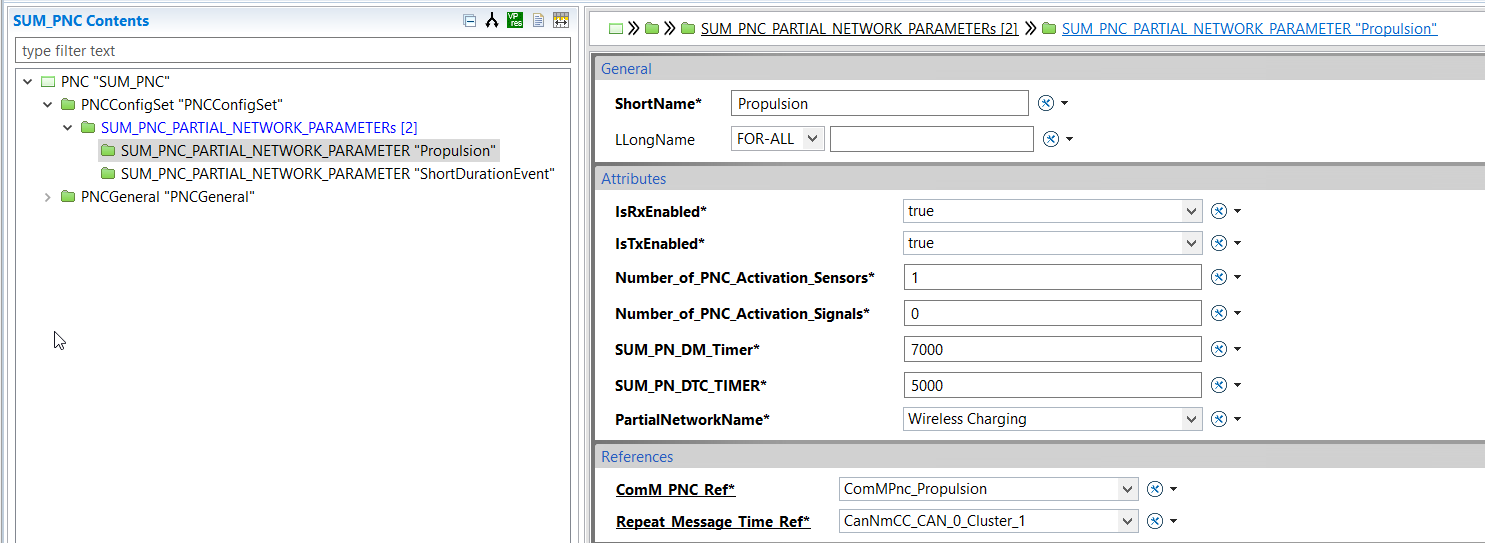
\includegraphics[width=\textwidth]{images/PNCConfigSet.png}
\caption{SUM\_PNC\_PARTIAL\_NETWORK\_PARAMETERS container.}\label{fig:PNCConfigSet}
\end{figure}

\textbf{IsRxEnabled }\newline
This parameter specifies if the RxPDU and RxPduGroup Interfaces are available for the PN or not. If TRUE, interfaces for SSFM and BswM will be created. 

\textbf{IsTxEnabled}\newline
This parameter specifies if the TxPDU and TxPduGroup Interfaces are available for the PN or not. If TRUE, interfaces for SSFM and BswM will be created.

\textbf{Number\_of\_PNC\_Activation\_Sensors}\newline
This parameter specifies the number of local sensor inputs contributing to the local activation criteria (\code{SUM\_PNC\_Criteria\_Sensor\_Act}) for this PN.

\textbf{Number\_of\_PNC\_Activation\_Signals}\newline
This parameter specifies the number of application signal inputs contributing to the local activation criteria (\code{SUM\_PNC\_Criteria\_Signal\_Act}) for this PN. Each signal has a corresponding status input (\code{SUM\_PNC\_Criteria\_SignalStat\_Act}); signal-based local activation requires BOTH \code{Signal\_Act} AND \code{SignalStat\_Act} to be TRUE. Note: These signals are evaluated locally on this ECU; remote PN activation is driven exclusively by NM frame reception via \code{PNC\_NM\_Frame\_Indication}.

\textbf{SUM\_PN\_DM\_Timer}\newline
This parameter specifies the time in milliseconds, for the PNC to request deactivation of the deadline monitoring associated with the Rx PDU group of each PN. 

\textbf{SUM\_PN\_DTC\_TIMER}\newline
This parameter is the initial value (in milliseconds) of the frequency for the SUM\_PN\_DTC\_TIMER. 

\textbf{ComM\_PNC\_Ref}\newline
Reference to the PN configuration in the ComM module.

\textbf{Repeat\_Message\_Time\_Ref}\newline
This parameter is the reference parameter for CanNmRepeatMessageTime (if CanNm is configured) or UdpNmRepeatMessageTime (if UdpNm is configured), which provides the Timeout for the Repeat Message State.
For ensuring the right computation, this value shall be expressed in milliseconds as all other configured timing values.

\textbf{PartialNetworkName}\newline
This parameter specifies the Name of the Partial Network, should be among the possible choices:
	0x21= All Nodes,
	0x22= Wireless Charging,
	0x23= Short Duration Event,
	0x24= Diagnose Mechatronics,
	0x25= Any Diagnose CAN PN.
This value is stored in \code{SUM\_PNC\_Cfg[n].PN\_Name} and is used as the NM remote activation wakeup reason. 

When a PN is remotely activated via \code{PNC\_NM\_Frame\_Indication}, its \code{PN\_Name} is added to the NM activation history, and \code{SUM\_PNC\_NM\_WR} is set to the minimum active PN name in that history.

\subsection{PNCGeneral}
\label{subsection:general}
This container (Figure~\ref{fig:PNCGeneral}) includes general parameters related to the entire PNC module.

\begin{figure}[htp]
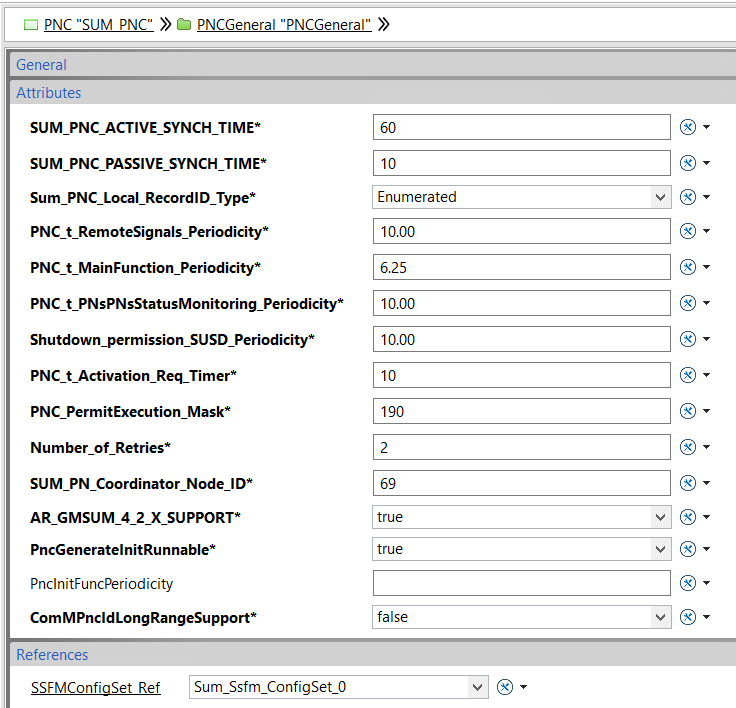
\includegraphics[width=\textwidth]{images/PNCGeneral.png}
\caption{PNCGeneral container.}\label{fig:PNCGeneral}
\end{figure}

\textbf{SUM\_PNC\_ACTIVE\_SYNCH\_TIME}\newline
This parameter specifies the time in milliseconds, for the PNC to request the PN Tx PDU group activation, after the activation of the Rx PDU group and after detecting that the activation criteria is met.

\textbf{SUM\_PNC\_PASSIVE\_SYNCH\_TIME}\newline
This parameter specifies the time in milliseconds, for the PNC to request the PN Tx PDU group activation, after the activation of the Rx PDU group and after detecting NM frame-based remote activation (via \code{PNC\_NM\_Frame\_Indication}).

\textbf{PNC\_t\_RemoteSignals\_Periodicity }\newline
This parameter specifies the time in milliseconds for the periodicity of polling for changes to the local activation signal inputs (\code{SUM\_PNC\_Criteria\_Signal\_Act}). Float values are supported. Note: Despite the parameter name, these signals contribute to local activation criteria; remote activation is driven by NM frame reception via \code{PNC\_NM\_Frame\_Indication}.

\textbf{PNC\_t\_MainFunction\_Periodicity}\newline
This parameter specifies the time in milliseconds for the periodicity of polling for changes to PNC state changes. Float values are supported.


\textbf{Shutdown\_permission\_SUSD\_Periodicity}\newline
This parameter specifies the time in milliseconds for the periodicity of Shutdown\_Permission runnable. Float values are supported. 


\textbf{PNC\_t\_Activation\_Req\_Timer }\newline
This parameter represents the time in milliseconds, to verify PN Activation after mode request (for retry purpose).

\textbf{PNC\_PermitExecution\_Mask}\newline
This paramater represents the mask that can be OR'd with the value supplied by PermitExecution to set any "don't care" bits to '1'.

\textbf{Number\_of\_Retries}\newline
This parameter indicates the number of retries.

\textbf{SUM\_PN\_Coordinator\_Node\_ID}\newline
This parameter represents the ECU ID (part of NM PDU) associated with CGM. It is checked in the function \code{PNC\_NM\_Frame\_Indication} to gate NM-driven remote activation processing: only NM frames whose source Node ID matches this value trigger remote activation and update the NM activation history (\code{SUM\_PNC\_NM\_WR}). It is also used for deadline monitoring control (used with \code{SUM\_PN\_n\_DM\_Timer}). Its value is expressed in DECIMAL. 


\textbf{AR\_GMSUM\_4\_2\_X\_SUPPORT }\newline
This parameter is used to distinguish between the AR ComM V4.0.3 and V4.1.1 and above. If AR ComM V4.0.3 is used, ComMPncId will be configured in range of 0-47, for V4.1.1 and above, the range is 8-63. 

\textbf{PncGenerateInitRunnable}\newline
It allows the generation of a periodic runnable to run function SUM\_PNC\_Init only the first time it is invoked.

\textbf{PncInitFuncPeriodicity}\newline
This parameter specifies the periodicity, in milliseconds, of the inizialization runnable. This parameter must be set when the configuration parameter PncGenerateInitRunnable is set to true.

\textbf{RTEVersion5x}\newline
In order to enable additional calls to access calibration parameters, this parameter is used to check if the RTE version is 5.x .

\textbf{ComMPncIdLongRangeSupport}\newline
This parameter is used to distinguish the range values that can be assigned to ComMPncId. If it is true the first comMPncId starts from 0, otherwise it starts from 16.
\\
\\
This means that if for instance the ComMPncId is in range $[$0, 255$]$ then this parameter shall be set to true.

\textbf{SSFMConfigSet\_Ref}\newline
Reference to the container SSFMConfigSet of the SSFM.

\subsubsection{PNCGeneral/ComM\_PNC\_Channel}
This container shall include the list of all ComM channels configured in the system.

\textbf{CAN\_Channel\_Number}\newline
This parameter will configure the CAN number with associated ComM channel reference. This parameter shall be used for updating Correct CAN channel status onto DID F08C.

\textbf{ComM\_Channel\_Ref}\newline
This parameter represents the ComM channel reference.

\textbf{Sum\_PNC\_Local\_RecordID\_Type}\newline 
This parameter will be used to indicate the record store type for local PN.

\section{Configuration Hints}

\subsection{Ports Name}
Be aware that after the generation of this module some ports have changed their name, you need to reconnect them. The ports whose name was composed using the PN ID of the PN are now composed using its ShortName.

\subsection{PN Number identification}
Depending on the boolean configuration parameter \textbf{AR\_GMSUM\_4\_2\_X\_SUPPORT}, in the container \textit{PNCGeneral}, a different PN configuration is expected :
\begin{itemize}
  \item \textbf{TRUE}  Unique 6 Byte ComSignal for partial networking
  \item \textbf{FALSE} One bit signal for each partial network
\end{itemize}

So, depending on this configuration, to retrieve the PN\_Number in the first case, the ComMPncId will be used, otherwise the ComBitPosition will be used.

\subsection{PN Deadline Monitoring Timer}
\label{subsec:dmTimer}
\begin{enumerate}
\item	Configure the DM parameters:
\item	The Configuration settings used by the DM are 2.
\begin{enumerate}
\item The first is \textbf{SUM\_PN\_Coordinator\_Node\_ID}, the ECU ID (part of NM PDU) associated with CGM that is used for deadline monitoring control (used with SUM\_PN\_n\_DM\_Timer). Value in DECIMAL. It is to be set under the module General container
\begin{center}
	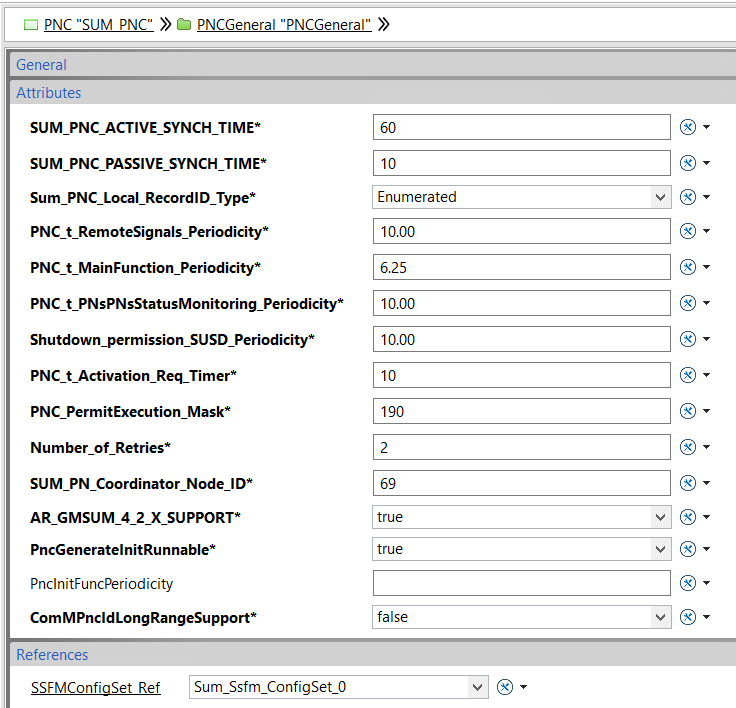
\includegraphics[width=0.6\textwidth]{images/PNCGeneral}
\end{center}
\item The second one is \textbf{SUM\_PN\_DM\_Timer}, the time in msec for the PNC to requestDeactivation of the deadline monitoring associated with Rx PDU group of each PN
\begin{center}
	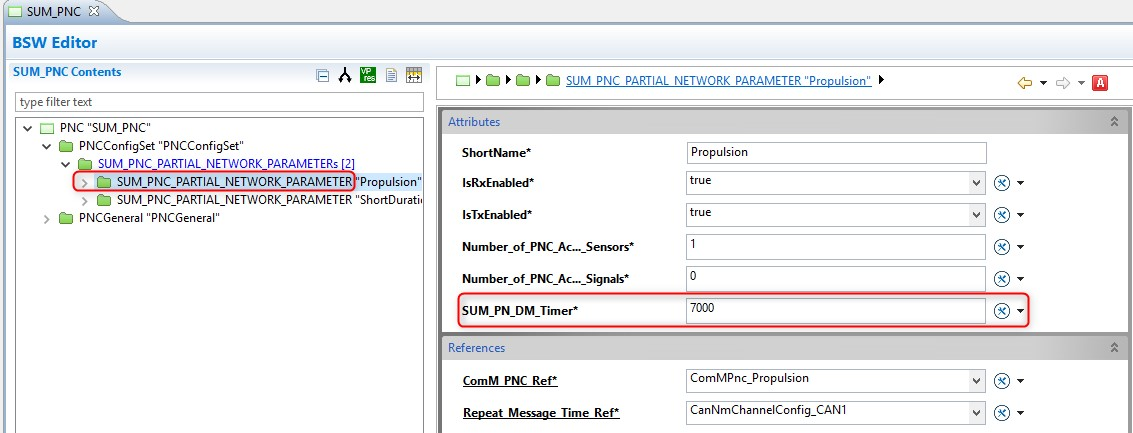
\includegraphics[width=0.6\textwidth]{images/PNParam}
\end{center}
\end{enumerate}
\item Regenerate the SUM PNC Module
\item Create in the BswM new DMC Action Items under the Mode Control, for enable and disable of each PN, and the necessary mode Request ports, LogicalExpression, ModeConditions, and Rules under the Arbitration container for each PN.
\begin{center}
	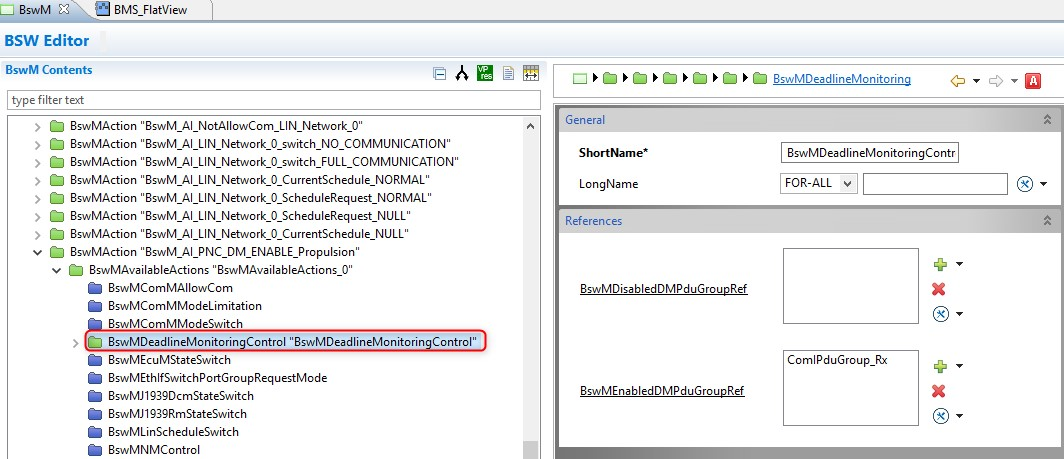
\includegraphics[width=0.6\textwidth]{images/BswMDeadline}
\end{center}
\item Connect the new interfaces available on the PNC to the BswM ones.
\paragraph{New Interfaces:} SUM PNC has a dedicated mode requester interface to request enabling (PN\_DM\_ENABLE) or disabling (PN\_DM\_DISABLE) the deadline monitoring for the PDU of the selected PN:
\input{generated/tables/interfaces.tex}
\item  Configure the parameter \textit{NmRxIndicationCallback} to the callback \textbf{PNC\_NM\_Frame\_Indication}, add \textbf{PNC.h} under \textit{NmRxCallbackHeader} in the Nm module and set to \textbf{true} \textit{NmPduRxIndicationEnabled}
\item  Configure to \textbf{true} \textit{CanNmPduRxIndicationEnabled} in the CanNm module
\item  Regenerate BSW
\item  Regenerate RTE
\end{enumerate}

Let's remember that the value of PN Deadline Monitoring Timer is a timing unit that shall be expressed in milliseconds. All configuration parameters for the configuration of periodicity are converted in micorseconds in  
code that is generated by scripts (\code{PNC\_Cfg.h} and \code{PNC\_Cfg.c}).

\subsection{PN DTC Timer}
\label{subsec:dtcTimer}
You need to set the following configuration parameter to allow RTA-SUM PNC to use the feature of the PN DTC Timer.
You had to configure a value for the timer for each PN.

\begin{center}
	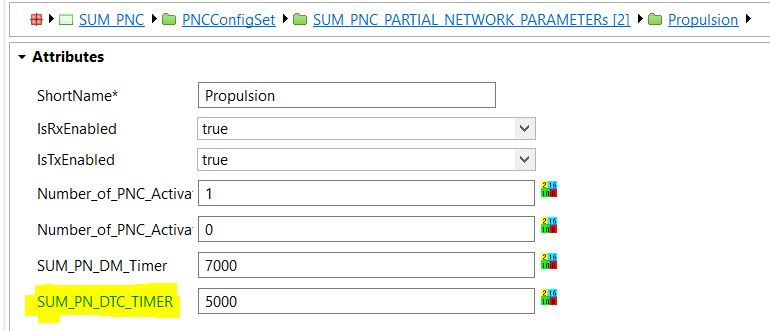
\includegraphics[width=0.6\textwidth]{images/dtct}
\end{center} 

Let's remember that the value of PN DTC Timer is a timing unit that shall be expressed in milliseconds. When its value is returned to PNC static code by functions, that are implemented in \code{PNC\_PBCfg.c} source
,it is converted in microsecond and it is stored in an \code{uint32} variable for computation. The conversion has been done in order to work only on integer values for computational part.


\subsection{Value of comMPncId}\label{subsection:commid}
The ComM module implementation by CUBAS has a limitation in the use case 'CBV + NodeId + Pnc Info', that is the one required by GM specifications.

The workaround suggested by CUBAS team is to configure the parameter \textbf{ComMPncId} of a PN in the container \textbf{ComM/ComMConfigSet} to \textit{<PNC-IDENTIFIER> - 8}.

This release of RTA-SUM PNC supports in parallel two use case:
\begin{itemize}
	\item CBV + NodeId + Pnc Info;
	\item CBV + Pnc Info;
\end{itemize}
For the second item the parameter \textbf{ComMPncId} of a PN is configured as \textit{<PNC-IDENTIFIER> - 16}.
\\
\\
The choice can be adoperated by dedicated configuration parameter in \ref{subsection:general} (PNC General)

\subsection{Ethernet ECUs and Conditional DID generation}
\label{subsection:EthernetECUDID}
Some ECUs types, as Ethernet ones, shall prevent the ports generation from PNC to Dcm as they are identified as "Conditional" in GM specification. The generation of ports, runnables and events for DIDs (Local and Remote) shall be supported in CAN ECUs only.

\subsection{Generation of a Periodic Runnable to run init function}
\label{subsection:generationrunnable}
If the requirements to meet ASIL D ask that a periodic runnable run the init function (SUM\_PNC\_Init), it is possible to generate this runnable by setting to true the configuration parameter \textit{PncGenerateInitRunnable} and specifying a periodicity (in milliseconds) in the \textit{PncInitFuncPeriodicity} configuration parameter. The generated runnable runs the SUM\_PNC\_Init function only the first time it is invoked.

\subsection{Disable PDU feature}
Feature included in the function Status\_PNC\_Tx\_Enable().
Every time PNC enables a PDU group, it also disables those PDUs of the group calibrated as disabled.

\subsubsection{SUM\_C\_Disable\_<n>}
Interface between SSFM and PNC, one instance for each PDU. 
Through these interfaces, PNC receives the calibration parameters that say if one PDU is disabled or not.

\subsubsection{SUM\_BswM\_DisablePdu}
It is an interface between the SUM\_PNC and the BswM. It exists one port instance implementing this interface for each PDU.\newline
From the BswM viewpoint, the user should manage this interface to implement a BswMModeRequestPort that triggers a BswMSwitchIPduMode action specific to each PDU.\newline
On the other hand, the SUM\_PNC uses these interfaces to request the PDU disabling, according to what it receives from the SUM\_SSFM.\newline
We guarantee proper behavior if the user takes the following actions:
\begin{itemize}
\item The user shall set the BswMRequestPort for the TxPduGroup as IMMEDIATE.
\item The user shall set the BswMRequestPort for the TxPduDisable as DEFERRED.
\end{itemize}.

\subsection{DID\_0xE0D7}
\label{subsection:0xE0D7}
The PNC shall utilize the SUSD\_PNC\_UpdateRecord interface to notify the SUSD of the activation or deactivation of a PN, specifying the type (local/remote) and the reason for the activation.
	
\begin{itemize}
\item For DID E0D7, choose a Partial Network from the list below only if needed; if not applicable, leave this field empty:
	\begin{itemize}
	\item All Nodes
	\item Wireless Charging
	\item Short Duration Event
	\item Diagnose Mechatronics
	\item Any Diagnose CAN PN
	\end{itemize}
    Example: If you configure a PartialNetworkName as "Wireless Charging", it will map directly to the Partial Network (PN) associated with wireless charging functionality.
\item The \code{Sum\_PNC\_Local\_RecordID\_Type} defines whether the Record ID for local activation is bitmapped or enumerated. Local activation include both sensors (\code{Number\_of\_PNC\_Activation\_Sensors}) and signals (\code{Number\_of\_PNC\_Activation\_Signals}), which are combined in a single unified history:
	\begin{itemize}
	\item In the bitmapped configuration, multiple local activation sources (sensors and signals) are reported simultaneously as bit flags
	(example: if Act\_Sensor\_CS0 = 0x1 and Act\_Signal\_S4 = 0x10, the combined value is 0x11).
	However, the total of \code{Number\_of\_PNC\_Activation\_Sensors} plus \code{Number\_of\_PNC\_Activation\_Signals} must not exceed 8 due to bit limitations.
	\item In the enumerated configuration, the lowest active local source (sensor or signal index) is given priority
	(example: if Act\_Sensor\_CS3 = 0x3 and Act\_Signal\_S4 = 0x4, 0x3 is prioritized).
	The total of \code{Number\_of\_PNC\_Activation\_Sensors} plus \code{Number\_of\_PNC\_Activation\_Signals} can not exceed 255 due to the 8-bit representation limitation.
	\item For NM frame-based remote activation, the Record ID is always enumerated and tracked separately via \code{SUM\_PNC\_NM\_WR}, recording the PN name of the remotely activating PN.
	\end{itemize}
\end{itemize}

\textbf{Note:} Only the "Any Diagnose CAN PN" option supports configuring for multiple Partial Networks. All other options allow only a single selection.